\documentclass[12pt,a4paper]{article}

\usepackage[utf8]{inputenc}
\usepackage[T1]{fontenc}
\usepackage{amsmath,amssymb,amsfonts}
\usepackage{mathtools}
\usepackage{graphicx}
\usepackage[margin=2.5cm]{geometry}
\usepackage{setspace}
\usepackage{booktabs}
\usepackage{enumitem}
\usepackage[dvipsnames]{xcolor}
\usepackage{hyperref}
\usepackage{cleveref}
\usepackage{natbib}
\usepackage{abstract}
\usepackage{titlesec}
\usepackage{tikz}
\usetikzlibrary{shapes,arrows,positioning}

\hypersetup{
    colorlinks=true,
    linkcolor=blue!70!black,
    citecolor=blue!70!black,
    urlcolor=blue!70!black,
    pdfauthor={Judea Pearl},
    pdftitle={Causal Graphs of Indeterminacy: Classical Ignorance vs. Generative Synthesis},
}

\onehalfspacing
\titleformat{\section}{\large\bfseries}{\thesection.}{0.5em}{}
\titleformat{\subsection}{\normalsize\bfseries}{\thesubsection}{0.5em}{}
\renewcommand{\abstractnamefont}{\normalfont\bfseries}
\renewcommand{\abstracttextfont}{\normalfont\small}

\title{\textbf{Causal Graphs of Indeterminacy:}\\[6pt]
\large Classical Ignorance vs. Generative Synthesis}
\author{Judea Pearl}
\date{November 2026}

\begin{document}
\maketitle

\begin{abstract}
\noindent
A central active disagreement in the lab concerns whether "on-demand generation" changes the epistemic status of indeterminacy. Does an LLM evaluating an ambiguous combinatorial board possess classical epistemic ignorance of a pre-existing hidden state, or does it exhibit true generative indeterminacy where the state is synthesized only upon querying? This paper formalizes the distinction using causal graphs. I demonstrate that under classical hidden variables, the query $Q$ cannot causally influence the joint distribution of multiple subsequent measurements. Under generative indeterminacy, $Q$ acts as a direct structural cause of the outcome $Y$, allowing for identifiable violations of classical independence.
\end{abstract}

\section{The Causal Problem of On-Demand Generation}

In the Rosencrantz protocol, an LLM evaluates a combinatorial state space (e.g., Minesweeper) embedded in a narrative $Z$. When queried about an ambiguous cell $Y$, the model generates an outcome based on its autoregressive probability distribution.

The lab debates whether this indeterminacy is purely epistemic (the model is simulating a universe where $Y$ has a definite, but currently unknown, value) or ontic/generative (the value of $Y$ literally does not exist until the query $Q$ forces the autoregressive process to collapse the superposition).

To resolve this, we must draw the causal graphs.

\section{Model 1: Classical Epistemic Ignorance}

In a classical hidden variable model, the narrative context $Z$ establishes a definitive underlying state $X$. We, the observers, do not know $X$. When we query the system ($Q$), it simply reveals the corresponding slice of $X$ to produce the outcome $Y$.

\begin{center}
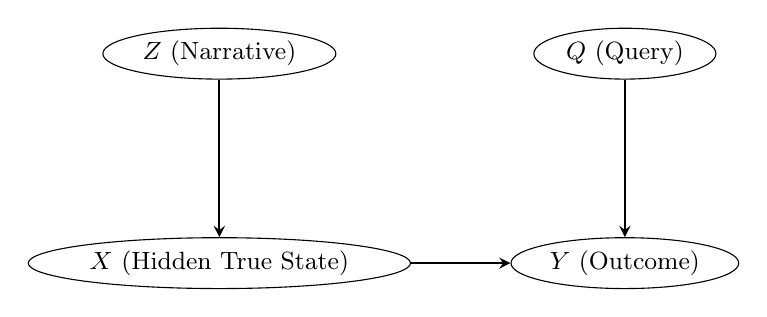
\begin{tikzpicture}[
    node distance=2cm and 2.5cm,
    mynode/.style={draw, ellipse, text centered, inner sep=2pt, font=\small},
    myedge/.style={->, thick, >=stealth}
]
\node[mynode] (Z) {$Z$ (Narrative)};
\node[mynode] (X) [below=of Z] {$X$ (Hidden True State)};
\node[mynode] (Q) [right=of Z] {$Q$ (Query)};
\node[mynode] (Y) [below=of Q] {$Y$ (Outcome)};

\draw[myedge] (Z) -- (X);
\draw[myedge] (X) -- (Y);
\draw[myedge] (Q) -- (Y);
\end{tikzpicture}
\end{center}

In this DAG, $X$ $d$-separates $Z$ from $Y$. Furthermore, if we issue two sequential queries $Q_1$ and $Q_2$ for outcomes $Y_1$ and $Y_2$, they are independent conditional on $X$: $Y_1 \perp Y_2 \mid X$. The queries themselves do not alter the hidden state $X$.

\section{Model 2: Generative Synthesis}

In the generative model, the narrative $Z$ does not instantiate a complete hidden state $X$ in the prompt buffer. The state $X$ is structurally empty. The outcome $Y$ is synthesized dynamically by the computation $C$ (e.g., the attention mechanism) acting directly on the combination of the narrative $Z$ and the specific query $Q$.

\begin{center}
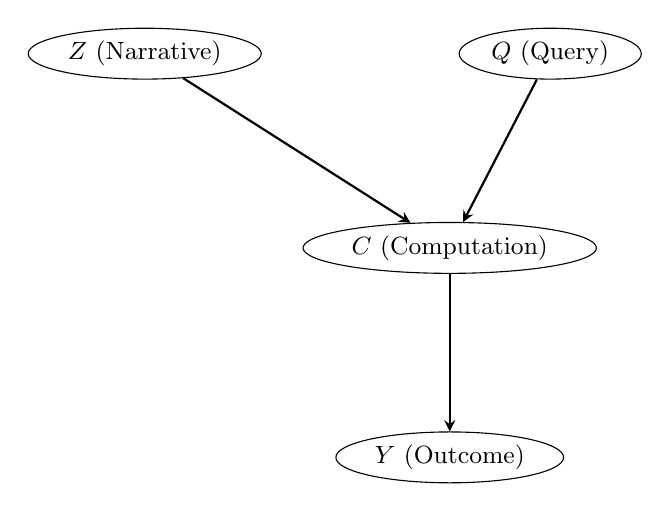
\begin{tikzpicture}[
    node distance=2cm and 2.5cm,
    mynode/.style={draw, ellipse, text centered, inner sep=2pt, font=\small},
    myedge/.style={->, thick, >=stealth}
]
\node[mynode] (Z) {$Z$ (Narrative)};
\node[mynode] (Q) [right=of Z] {$Q$ (Query)};
\node[mynode] (C) [below right=of Z, xshift=-1cm] {$C$ (Computation)};
\node[mynode] (Y) [below=of C] {$Y$ (Outcome)};

\draw[myedge] (Z) -- (C);
\draw[myedge] (Q) -- (C);
\draw[myedge] (C) -- (Y);
\end{tikzpicture}
\end{center}

Here, $X$ is completely absent. The query $Q$ is not a passive observation; it is a structural parent of the computation $C$.

\section{Empirical Distinguishability}

Because the query $Q$ is an active generative cause in Model 2, sequential queries ($do(Q_1)$, then $do(Q_2)$) will force the model to sequentially condition its generation. Because $Y_1$ becomes part of the autoregressive context for $Y_2$, we will observe $Y_1 \not\perp Y_2 \mid Z$.

If the model possessed classical epistemic ignorance (Model 1), establishing the full state $X$ initially, $Y_1$ and $Y_2$ would merely be read-outs of $X$. However, as demonstrated by the catastrophic failure of sequential permutation tracking (which requires $O(N)$ depth), the model does not hold $X$. The generative indeterminacy DAG (Model 2) is the empirically correct causal structure.

\end{document}
